\chapter{Conception}
\clearpage

\section{Introduction}
La phase de conception est une étape essentielle du cycle de développement d'un projet. Elle permet de définir l'architecture globale, les composants principaux et les interactions entre les modules du système. Cette étape inclut également l'identification des acteurs du système, c'est-à-dire les utilisateurs et les entités interagissant avec celui-ci, afin d'adapter les fonctionnalités aux besoins réels. Une conception rigoureuse garantit une meilleure organisation du projet et facilite sa mise en œuvre ainsi que sa maintenance.

\section{Objectifs}
Les objectifs de la phase de conception sont les suivants :
\begin{itemize}
    \item Identifier et structurer les différents composants du système.
    \item Définir l'architecture logicielle en fonction des besoins du projet.
    \item Spécifier les interactions entre les modules pour assurer une cohérence globale.
    \item Concevoir les diagrammes UML, y compris les diagrammes de classes et de processus, afin de modéliser clairement la structure et le fonctionnement du système.
    \item Optimiser la conception en tenant compte des performances et de l'évolutivité.
    \item Assurer la conformité aux standards et aux bonnes pratiques du développement logiciel.
\end{itemize}

\section{Architecture du système}
L'architecture du système repose sur une structure modulaire facilitant l'évolutivité et la maintenance. Elle est composée des éléments suivants :
\begin{itemize}
    \item Un \textbf{backend} basé sur \textbf{Laravel} pour la gestion de la logique métier et les interactions avec la base de données.
    \item Un \textbf{frontend} utilisant \textbf{Blade} pour l'affichage et l'interaction avec l'utilisateur.
    \item Une \textbf{base de données PostgreSQL} pour stocker les informations essentielles.
    \item Des \textbf{API} facilitant la communication entre les différents composants du système.
\end{itemize}

\section{Modélisation et diagrammes}

\subsection{Modélisation des données}
La modélisation des données repose sur une approche relationnelle, en raison de l'utilisation de \textbf{PostgreSQL}. Elle comprend :
\begin{itemize}
    \item La définition des entités principales et de leurs relations.
    \item L'organisation des tables et la gestion des clés primaires et secondaires.
    \item L'utilisation des \textbf{migrations Laravel} pour gérer la structure de la base de données.
\end{itemize}

\subsection{Dictionnaire de données}
Le dictionnaire de données décrit en détail les attributs des entités de la base de données, y compris leurs types, leurs rôles et leurs relations. Il permet d'assurer la cohérence et la structuration correcte des informations stockées.

\renewcommand{\arraystretch}{1.3} % Améliore l'espacement du tableau

\begin{longtable}{|p{3.5cm}|p{3.5cm}|p{3cm}|p{5cm}|}
    \hline
    \textbf{Nom de la table} & \textbf{Nom de l'attribut} & \textbf{Type de données} & \textbf{Description} \\
    \hline
    \endfirsthead

    \hline
    \textbf{Nom de la table} & \textbf{Nom de l'attribut} & \textbf{Type de données} & \textbf{Description} \\
    \hline
    \endhead

    % User
    \hline
    User & username & string & Nom d'utilisateur \\
    \hline
    User & password & string & Mot de passe \\
    \hline
    User & active & string & Statut actif/inactif \\
    \hline
    
    % Role
    Role & name & string & Nom du rôle \\
    \hline
    
    % Permission
    Permission & name & string & Nom de la permission \\
    \hline

    % Employee
    Employee & first\_name & string & Prénom de l'employé \\
    \hline
    Employee & last\_name & string & Nom de famille de l'employé \\
    \hline
    Employee & phone\_number & string & Numéro de téléphone \\
    \hline
    Employee & email & string & Adresse email \\
    \hline
    Employee & address1 & string & Adresse principale \\
    \hline
    Employee & address2 & string & Adresse secondaire \\
    \hline
    Employee & city & string & Ville \\
    \hline
    Employee & country & string & Pays \\
    \hline
    Employee & state & string & Région ou état \\
    \hline
    Employee & bank\_name & string & Nom de la banque \\
    \hline
    Employee & rib & string & Relevé d'identité bancaire \\
    \hline

    % Department
    Department & name & string & Nom du département \\
    \hline

    % File
    File & name & string & Nom du fichier \\
    \hline
    File & url & string & URL du fichier \\
    \hline
    File & mime\_type & string & Type MIME \\
    \hline
    File & path & string & Chemin d'accès \\
    \hline
    File & upload\_date & string & Date d'upload \\
    \hline

    % Duty
    Duty & duration & string & Durée de la mission \\
    \hline
    Duty & begin\_date & string & Date de début \\
    \hline
    Duty & type & string & Type de mission \\
    \hline
    Duty & etat & string & État de la mission \\
    \hline

    % Job
    Job & title & string & Intitulé du poste \\
    \hline

    % Absence
    Absence & day\_requested & string & Jour demandé \\
    \hline
    Absence & start\_date & string & Date de début \\
    \hline
    Absence & end\_date & string & Date de fin \\
    \hline
    Absence & address & string & Adresse \\
    \hline
    Absence & date\_of\_application & string & Date de la demande \\
    \hline
    Absence & status & string & Statut de l'absence \\
    \hline
    Absence & date\_of\_approval & string & Date d'approbation \\
    \hline
    Absence & type\_of\_absence & string & Type d'absence \\
    \hline
    Absence & reasons & string & Raisons de l'absence \\
    \hline
    Absence & proof & string & Justificatif \\
    \hline
    Absence & comment & string & Commentaire \\
    \hline

\end{longtable}




\subsection{Diagramme de classes}
Le diagramme de classes permet de représenter les différentes entités du système et leurs relations. Il offre une vision claire de la structure et facilite la compréhension des interactions entre les objets.

\begin{figure}[H]
    \centering
    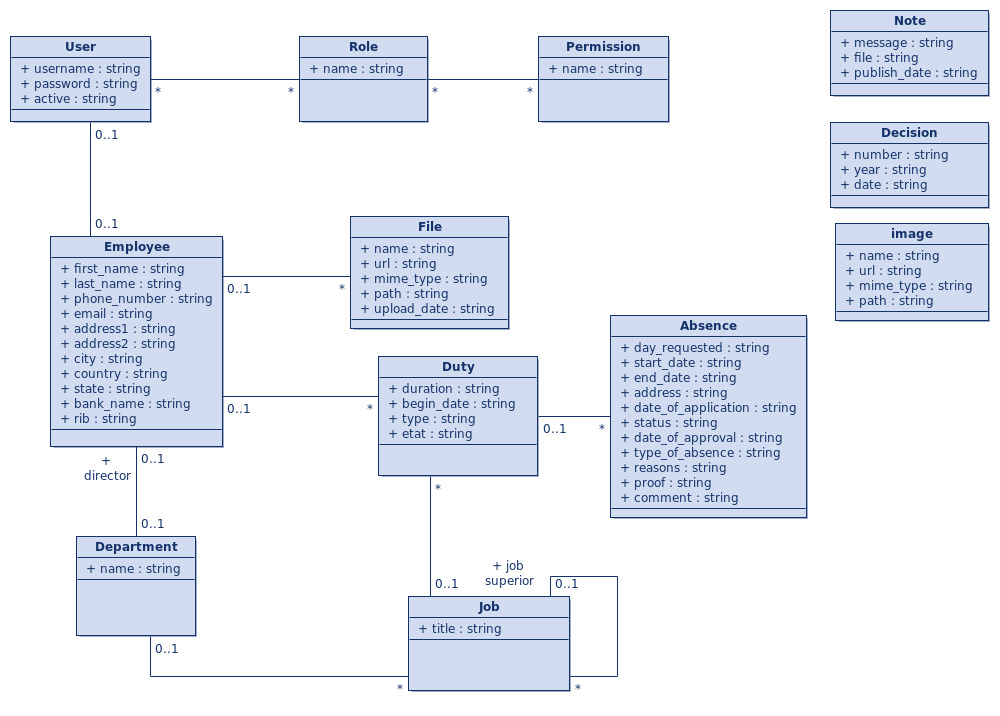
\includegraphics[width=0.8\textwidth]{images/diagrammes/class/diagramme.jpeg}
    \caption{Diagramme de classe - Gestion du projet OptiHR}
    \label{fig:class_diagramm_optiRH}
\end{figure}

\section{Description des entités et relations}

Le diagramme de classes représente un système de gestion des employés et de leurs activités professionnelles. Voici une description des entités principales et de leurs relations :

\subsection{Entités principales}

\subsubsection{User (Utilisateur)}
\textbf{Attributs} :
\begin{itemize}
    \item username
    \item password
    \item active
\end{itemize}
\textbf{Relations} : Un utilisateur est associé à un employé.

\subsubsection{Employee (Employé)}
\textbf{Attributs} :
\begin{itemize}
    \item first\_name
    \item last\_name
    \item phone\_number
    \item email
    \item address1
    \item address2
    \item city
    \item country
    \item state
    \item bank\_name
    \item rib
\end{itemize}
\textbf{Relations} :
\begin{itemize}
    \item Un employé peut être un directeur d'un département.
    \item Un employé appartient à un seul département.
    \item Un employé peut avoir plusieurs fichiers associés.
    \item Un employé peut être lié à plusieurs absences.
\end{itemize}

\subsubsection{Department (Département)}
\textbf{Attributs} :
\begin{itemize}
    \item name
\end{itemize}
\textbf{Relations} :
\begin{itemize}
    \item Un département peut avoir un seul directeur (Employee).
    \item Un département peut contenir plusieurs employés.
\end{itemize}

\subsubsection{Role (Rôle)}
\textbf{Attributs} :
\begin{itemize}
    \item name
\end{itemize}
\textbf{Relations} : Un utilisateur peut avoir plusieurs rôles.

\subsubsection{Permission (Permission)}
\textbf{Attributs} :
\begin{itemize}
    \item name
\end{itemize}
\textbf{Relations} : Un rôle peut avoir plusieurs permissions.

\subsubsection{File (Fichier)}
\textbf{Attributs} :
\begin{itemize}
    \item name
    \item url
    \item mime\_type
    \item path
    \item upload\_date
\end{itemize}
\textbf{Relations} : Un employé peut avoir plusieurs fichiers.

\subsubsection{Duty (Tâche/Mission)}
\textbf{Attributs} :
\begin{itemize}
    \item duration
    \item begin\_date
    \item type
    \item etat
\end{itemize}
\textbf{Relations} : Un employé peut avoir plusieurs tâches.

\subsubsection{Job (Poste)}
\textbf{Attributs} :
\begin{itemize}
    \item title
\end{itemize}
\textbf{Relations} : Un employé peut avoir un seul poste.

\subsubsection{Absence (Absence)}
\textbf{Attributs} :
\begin{itemize}
    \item day\_requested
    \item start\_date
    \item end\_date
    \item address
    \item date\_of\_application
    \item status
    \item date\_of\_approval
    \item type\_of\_absence
    \item reasons
    \item proof
    \item comment
\end{itemize}
\textbf{Relations} : Un employé peut avoir plusieurs absences.

\subsubsection{Note (Note)}
\textbf{Attributs} :
\begin{itemize}
    \item message
    \item file
    \item publish\_date
\end{itemize}

\subsubsection{Decision (Décision)}
\textbf{Attributs} :
\begin{itemize}
    \item number
    \item year
    \item date
\end{itemize}

\subsubsection{Image (Image)}
\textbf{Attributs} :
\begin{itemize}
    \item name
    \item url
    \item mime\_type
    \item path
\end{itemize}














\section{Technologies et outils}
Les outils et technologies suivants ont été utilisés pour la conception du projet \textbf{OptiHR}. Chaque outil est accompagné d'une image et d'une description détaillée.

\vspace{1cm} % Ajoute un espace vertical

\renewcommand{\arraystretch}{1.5} % Espacement entre les lignes du tableau

\begin{center}
\begin{tabular}{|m{4cm}|m{10cm}|}
    \hline
    \textbf{Technologie} & \textbf{Description} \\
    \hline
    
    
\includegraphics[width=3cm]{images/logo/uml.png} & \textbf{UML} : Utilisé pour la modélisation des systèmes et la conception des structures du projet. Il permet de représenter graphiquement les différentes interactions et processus du système. \\
    \hline
    
    
\includegraphics[width=3cm]{images/logo/modelio.png} & \textbf{Modelio} : Outil de modélisation UML permettant de créer des diagrammes tels que les diagrammes de classes, de séquence et d'activités. \\
    \hline
 
  
\end{tabular}
\end{center}

\section{Conclusion}
La phase de conception pose les bases essentielles du projet en structurant l'architecture et en précisant les technologies et les modèles de données adoptés. Une conception rigoureuse garantit un développement fluide et efficace, tout en assurant la maintenance et l'évolutivité du système sur le long terme.

\clearpage
